\documentclass[conference]{IEEEtran}
\IEEEoverridecommandlockouts

\usepackage{cite}
\usepackage{amsmath,amssymb,amsfonts}
\usepackage{algorithm}
\usepackage{algorithmic}
\usepackage{graphicx}
\usepackage{booktabs}
\usepackage{textcomp}
\usepackage{xcolor}
\usepackage{listings}
\usepackage{tikz}
\usepackage{pgfplots}
\pgfplotsset{compat=1.17}
\usetikzlibrary{arrows.meta,positioning,shapes.geometric,fit,backgrounds,calc}

\def\BibTeX{{\rm B\kern-.05em{\sc i\kern-.025em b}\kern-.08em
    T\kern-.1667em\lower.7ex\hbox{E}\kern-.125emX}}

% ---- listing style ----
\definecolor{codebg}{RGB}{247,247,249}
\definecolor{kw}{RGB}{34,34,110}
\definecolor{cmt}{RGB}{90,120,90}
\definecolor{str}{RGB}{150,60,40}
\lstset{
  basicstyle=\ttfamily\scriptsize,
  backgroundcolor=\color{codebg},
  keywordstyle=\color{kw}\bfseries,
  commentstyle=\color{cmt}\itshape,
  stringstyle=\color{str},
  breaklines=true,
  columns=fullflexible,
  showstringspaces=false,
  frame=single,
  framesep=4pt,
  aboveskip=6pt,belowskip=4pt,
  xleftmargin=4pt,xrightmargin=2pt,
}

% ---- TikZ shared styles ----
\tikzset{
  box/.style={rectangle, rounded corners=2pt, draw=black!70, thick,
    align=center, font=\scriptsize, inner sep=3pt, minimum height=7mm},
  scaff/.style={box, fill=blue!10},
  net/.style={box, fill=green!12},
  obs/.style={box, fill=violet!12},
  store/.style={box, fill=orange!12},
  client/.style={box, fill=black!6},
  decision/.style={diamond, aspect=2, draw=black!70, thick, fill=yellow!15,
    align=center, font=\scriptsize, inner sep=1pt},
  term/.style={rectangle, rounded corners=6pt, draw=black!70, thick,
    align=center, font=\scriptsize\bfseries, inner sep=3pt, minimum height=6mm},
  flow/.style={-{Stealth[length=2mm]}, thick},
  flowd/.style={-{Stealth[length=2mm]}, thick, dashed},
}

\begin{document}

\title{Weblay: Persistent Overlay Visual Editing of Evolving Web Pages via Multi-Signal Element Anchoring}

\author{\IEEEauthorblockN{Sathnindu Kottage}
\IEEEauthorblockA{\textit{Faculty of Computing} \\
\textit{Sri Lanka Institute of Information Technology}\\
Malabe, Sri Lanka \\
it22602282@my.sliit.lk}}

\maketitle

% Abstract and keywords typeset manually (not via the IEEEtran abstract/
% IEEEkeywords environments) so the run-in label uses a colon rather than the
% class's built-in em dash.
\vspace{2pt}
\noindent{\footnotesize\textbf{\textit{Abstract}:} Maintaining persistent end-user visual modifications on deployed web pages necessitates the reliable identification of edited elements as underlying markup evolves. Conventional overlay-based visual editors anchor modifications to singular CSS selectors, an approach that fails upon markup alteration and typically provides no indication of application failure. This paper presents a methodology associating each edit with a multi-signal element descriptor comprising an authored anchor, a trusted-identifier path, a structural path, and a content fingerprint. This descriptor is re-resolved server-side against newly fetched HTML using a hashing procedure identical to the browser-side mechanism. The re-resolution outcome is classified into one of six change categories. Three independent detection channels, specifically bind-time risk assessment, periodic crawling, and runtime visitor telemetry, generate a composite confidence score and a four-state status. Additionally, a mass-drift heuristic distinguishes incremental alterations from comprehensive redesigns. Each change category corresponds to a specific corrective action: a non-destructive original page preview, per-element restoration, re-binding, or hardening. This approach is implemented in Weblay, a system delivered via a single \texttt{<script>} tag utilizing a 4.9\,KB gzipped runtime and a lazily loaded editor isolated within a Shadow DOM. In an end-to-end evaluation on a representative multi-section site, all six categories were accurately classified across fifteen seeded edits, yielding no false positives on the unchanged set. Every flagged edit was successfully resolved via its prescribed action, reducing the outstanding-issue count to zero. The software architecture comprises 5{,}664 lines of Go leveraging a three-backend storage abstraction, alongside a 4{,}947-line TypeScript client.\par}

\vspace{4pt}
\noindent{\footnotesize\textbf{\textit{Keywords}:} visual web editing, DOM anchoring, content drift, selector robustness, in-place editing, live websites\par}
\vspace{6pt}

\section{Introduction}
Modifying the visible content of production websites incurs overhead that is often disproportionate to the magnitude of the alteration. Minor modifications, such as single-word text corrections or image replacements, typically necessitate source-code modifications, pull requests, continuous-integration builds, and subsequent redeployments. While content-management systems (CMS) eliminate direct developer involvement in this cycle, they primarily benefit architectures initially designed around them. Integrating a CMS into a preexisting static or server-rendered architecture constitutes a substantial migration effort. Consequently, routine content maintenance remains dependent on engineering availability, frequently delaying minor, time-sensitive corrections until development resources are allocated.

Overlay visual editors offer an intermediary solution by injecting a lightweight script into unmanaged pages, enabling non-technical users to modify elements directly and propagating these modifications to subsequent visitors. This paradigm, utilized by commercial A/B-testing and personalization platforms, exhibits a fundamental vulnerability in element anchoring. Edits are typically bound to a CSS selector or XPath captured during the initial modification. Consequently, minor markup alterations during subsequent deployments can cause the selector to resolve incorrectly, redundantly, or fail entirely. This results in misapplied, duplicated, or omitted edits. Furthermore, operators lack visibility into these failures, as the systems assume the persistent validity of stored selectors. Because such failures occur silently, misapplied or omitted edits may persist across multiple subsequent deployments before detection; furthermore, manually re-auditing every stored selector following each release scales poorly with edit volume and deployment frequency.

This paper introduces a method for maintaining the correct location of end-user visual edits on deployed web pages during underlying markup evolution, accompanied by a mechanism for detecting and classifying instances where edits become unlocatable. This approach is implemented in a system designated as Weblay. The primary contributions are: (1) a single-tag delivery model featuring a 4.9 KB gzipped visitor runtime that applies published edits without framework dependencies, alongside a 29 KB lazily loaded editor restricted to authorized users, with all editor chrome rendered within a Shadow DOM; (2) a multi-signal element descriptor recording an authored data-weblay anchor, a trusted-identifier path, a structural nth-of-type path, and a content or attribute fingerprint for each edit; (3) a server-side re-anchoring and classification engine that re-resolves descriptors against newly crawled HTML to assign one of six change categories, utilizing a hashing implementation identical to that of the browser; (4) three complementary detection channels (bind-time risk, authoritative crawling, and privacy-preserving runtime telemetry) that inform a confidence score, a four-state health ladder, and a mass-drift heuristic; and (5) a guided recovery model pairing each categorization with a corresponding corrective action.

\begin{enumerate}
\item \textbf{A single-tag delivery model} in which a 4.9\,KB gzipped visitor runtime applies published edits with no framework dependency, and a 29\,KB editor is lazily loaded only when an edit grant is present. All editor chrome renders inside a Shadow DOM, so it cannot collide with or be styled by the host page.
\item \textbf{A multi-signal element descriptor} that records, for every edit, an authored \texttt{data-weblay} anchor, a trusted-identifier path, a structural nth-of-type path, and a content/attribute fingerprint, so that no single fragile selector stands between an edit and its element.
\item \textbf{A server-side re-anchoring and classification engine} that re-resolves each descriptor against freshly crawled HTML and assigns one of six change categories (unchanged, moved, content-conflict, replaced, removed, ambiguous), using a hashing implementation that is byte-for-byte identical to the browser's so that a descriptor captured in the page re-resolves the same way on the server.
\item \textbf{Three complementary detection channels} (bind-time risk assessment, an authoritative periodic crawl, and privacy-preserving runtime telemetry) feeding a confidence score, a four-state health ladder (healthy, at-risk, broken, quarantined), and a mass-drift heuristic that recognizes a whole-page redesign rather than raising a hundred independent alarms.
\item \textbf{A guided recovery model} that pairs each category with a safe corrective action: a non-destructive \emph{peek} at the original page, a per-element \emph{reset}, a \emph{re-bind} that re-anchors an edit onto a moved element, and \emph{hardening} that adds a durable authored anchor.
\end{enumerate}

The remainder of this paper is organized as follows. Section II reviews related literature regarding visual editing and element-locator robustness. Section III details the methodology, encompassing the delivery and storage models, the multi-signal descriptor and its cross-environment re-resolution, the detection channels, the classification procedure, and the recovery actions. Section IV presents and discusses the results of an end-to-end system evaluation. Section V concludes the paper and outlines directions for future research.

\section{Literature Review}\label{sec:related}
\subsection{Visual and In-Place Editors}
Site builders such as Webflow [1] and the WordPress block editor [2] facilitate comprehensive visual editing by controlling the rendering pipeline of the page; content is maintained within their proprietary data models, and the resulting HTML is generated as output. Consequently, these tools are incompatible with preexisting sites supported by independent technology stacks. While headless and hybrid CMS architectures offer flexibility regarding the rendering location, they still necessitate that pages be authored in accordance with their specific content models.

\subsection{Overlay A/B and Personalization Tools}
Optimization platforms, including the visual editors integrated into A/B-testing suites [3], introduced script-tag overlay editing for live web pages. These systems store visual modifications as selector-scoped, client-side mutations. Operational reports concerning these tools frequently identify selector fragility across deployments as a primary cause of orphaned or erroneously applied variations. The proposed Weblay system adopts a similar non-invasive delivery mechanism but substitutes the single-selector anchor with a multi-signal descriptor, while also introducing explicit drift-detection and recovery layers absent in existing tools.

\subsection{Selector and Element-Identity Robustness}
Robust element location remains a persistent challenge in web test automation because locators frequently break during application evolution. Existing research on multi-locator [4] and robust XPath [5] strategies, along with self-healing tools like Healenium [6], aggregates multiple weak signals (such as attributes, text, structural position, and visual features) and utilizes a voting mechanism to withstand structural changes. Weblay adapts this methodology to the distinct context of persisted end-user edits. Instead of repairing a locator for an isolated test execution, the system determines offline and at scale whether a stored edit remains valid for a production page. If the edit is invalid, the system identifies the cause to determine the appropriate recovery action.

\subsection{DOM Comparison}
Tree-diffing algorithms for hierarchical documents [7] form the basis of virtual DOM reconciliation [8] and HTML change detection. Instead of performing full tree diffing, Weblay re-resolves individual descriptors and validates the results using content fingerprints. This approach maintains independent and computationally efficient per-element classification while facilitating page-level redesign assessments via a mass drift ratio.

\section{Methodology}\label{sec:method}
This section details the system architecture of Weblay. It outlines the delivery and storage models, the multi-signal element descriptor alongside its cross-environment re-resolution, the three detection channels, the classification procedure, and the corresponding recovery actions provided for each outcome.

\subsection{System Overview}
Fig.~\ref{fig:arch} shows the overall structure. A single script tag on the customer's page loads the visitor runtime, which fetches a cached JSON \emph{manifest} of published edits and applies them. When the page is opened with a short-lived edit grant, the runtime lazily loads the editor bundle. A Go server exposes the dashboard API, the edit-mode API, the public manifest, and asset uploads, and persists state through a storage abstraction with three interchangeable backends. A background crawler periodically re-anchors every stored edit against the live site.

\begin{figure}[t]
\centering
\resizebox{\columnwidth}{!}{%
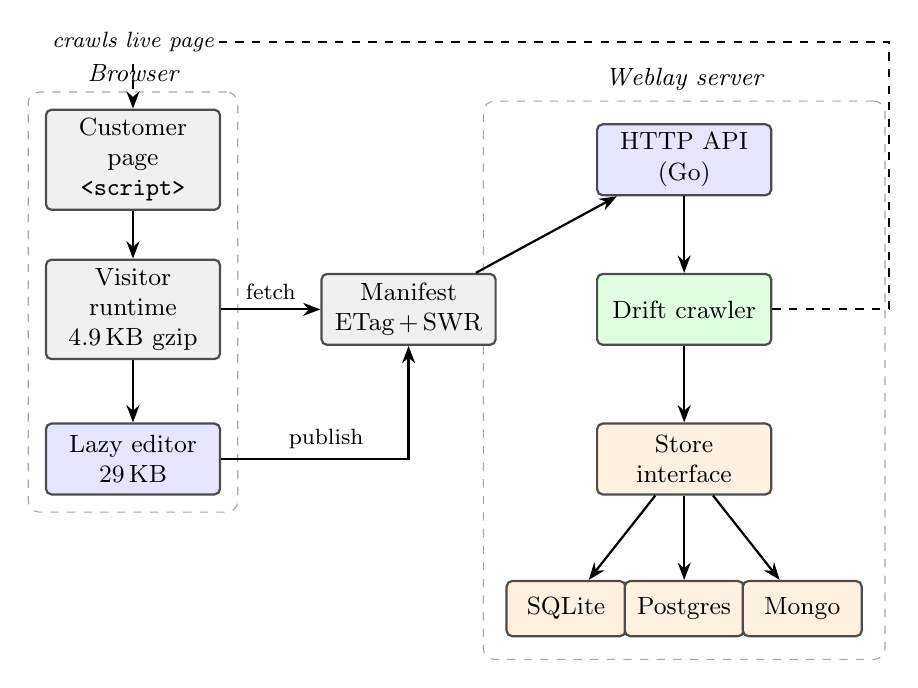
\begin{tikzpicture}[
  every node/.style={font=\small},
  b/.style={rectangle, rounded corners=2pt, draw=black!70, thick, align=center,
            inner sep=3pt, minimum height=9mm, text width=20mm},
  db/.style={b, fill=orange!12, text width=13mm, minimum height=7mm},
  flow/.style={-{Stealth[length=2.2mm]}, thick},
  flowd/.style={-{Stealth[length=2.2mm]}, thick, dashed},
]
% Browser column
\node[b, fill=black!6] (tag) at (0,0)      {Customer page \\ \texttt{<script>}};
\node[b, fill=black!6] (rt)  at (0,-1.9)   {Visitor runtime \\ 4.9\,KB gzip};
\node[b, fill=blue!10] (ed)  at (0,-3.8)   {Lazy editor \\ 29\,KB};
% Manifest bridge (aligned with visitor runtime)
\node[b, fill=black!6] (mani) at (3.5,-1.9) {Manifest \\ ETag\,+\,SWR};
% Server column
\node[b, fill=blue!10]   (api)   at (7.0,0)    {HTTP API \\ (Go)};
\node[b, fill=green!12]  (drift) at (7.0,-1.9) {Drift crawler};
\node[b, fill=orange!12] (store) at (7.0,-3.8) {Store interface};
% Databases
\node[db] (sqlite) at (5.5,-5.7) {SQLite};
\node[db] (pg)     at (7.0,-5.7) {Postgres};
\node[db] (mongo)  at (8.5,-5.7) {Mongo};
% Group frames
\begin{scope}[on background layer]
  \node[draw=black!35, dashed, rounded corners, fit=(tag)(ed), inner sep=6pt,
        label={[font=\small\itshape]above:Browser}] {};
  \node[draw=black!35, dashed, rounded corners, fit=(api)(sqlite)(mongo), inner sep=8pt,
        label={[font=\small\itshape]above:Weblay server}] {};
\end{scope}
% Data flow (no crossings)
\draw[flow] (tag) -- (rt);
\draw[flow] (rt)  -- (ed);
\draw[flow] (rt)  -- (mani) node[midway, above, font=\footnotesize] {fetch};
\draw[flow] (mani) -- (api);
\draw[flow] (ed.east) -| (mani.south) node[pos=0.28, above, font=\footnotesize] {publish};
\draw[flow] (api)   -- (drift);
\draw[flow] (drift) -- (store);
\draw[flow] (store) -- (sqlite);
\draw[flow] (store) -- (pg);
\draw[flow] (store) -- (mongo);
% Crawl feedback routed around the right and across the top (no crossings)
\draw[flowd] (drift.east) -| (9.6,1.5) -| (tag.north)
      node[pos=0.5, fill=white, inner sep=1.5pt, font=\footnotesize\itshape] {crawls live page};
\end{tikzpicture}}
\caption{Weblay architecture. A single script tag loads the visitor runtime, which applies a cached manifest and lazily loads the Shadow-DOM editor. The Go server re-anchors edits against the live page (dashed) through a background crawler.}
\label{fig:arch}
\end{figure}

\subsection{Delivery Model}
The connector is developed in TypeScript and compiled into two immediately invoked functions. The visitor bundle, designated as weblay.js (12.3 KB raw, 4.9 KB gzipped), executes on every page load to retrieve the manifest and apply published overrides. The editor bundle, designated as weblay-editor.js (112 KB raw, 29 KB gzipped), is retrieved exclusively when an edit token exists in the URL fragment, preventing unnecessary downloads for standard visitors. Because this token resides in the URL fragment rather than the query string, it is never transmitted to the server with the page request. The complete editor user interface, including toolbars, the layers panel, and floating property panels, is encapsulated within a Shadow DOM [9] attached to the top document. This encapsulation prevents cascading style sheet interference between the host page and the editor in both directions. For responsive previews, the page is embedded within an iframe device stage to ensure media queries are evaluated against an accurate viewport width.

\subsection{Override Representation}
An edit is persisted as an override, functioning as a record indexed by the element selector. This record contains an ElementContent value alongside optional fields for text, sanitized HTML, attributes, inline styles, and per-breakpoint media styles. The published overrides for a page are aggregated into a single manifest. This manifest is served with an ETag, a 30-second max-age directive, and a 300-second stale-while-revalidate window [11]. Consequently, the visitor runtime applies edits asynchronously, avoiding network blocking during standard execution paths.

\subsection{Storage Abstraction}
Data persistence is abstracted through a unified Store interface featuring two distinct implementations: a SQL store supporting SQLite via a pure Go driver and PostgreSQL, and a document store for MongoDB. This architecture permits the server to operate using a zero-configuration local SQLite file during development and a managed PostgreSQL or MongoDB cluster in production environments without requiring source code modifications. Entities including health records, overrides, revisions, assets, sites, and users are defined singularly at the interface level and are supported equivalently by both database backends.

\subsection{Security Boundaries}
The system treats the browser as an untrusted environment. Server-side HTML sanitization functions as an independent trust boundary, distinct from client-side processes, ensuring that manifested content remains secure irrespective of editor submissions. Edit-mode requests utilize a short-lived bearer token and adhere to per-site cross-origin constraints. The public manifest and telemetry endpoints permit cross-origin reads without conferring authority. Runtime telemetry transmits an opaque beacon comprising structural selectors and state codes, strictly excluding page content.

\subsection{The Multi-Signal Descriptor}\label{sec:drift}
Conventional overlay editors typically anchor modifications to a single structural selector, a method susceptible to markup mutations. Alternatively, the proposed technique records a composite descriptor at bind time, comprising multiple independent signals (Listing 1). These signals include an authored data-weblay attribute if available as the primary author-controlled anchor, a path relative to the nearest trusted non-generated element identifier, a structural nth-of-type path, and a multipoint fingerprint. This fingerprint incorporates the tag name, a normalized text hash, a stable attribute signature hash, the sibling index, and the nearest semantic landmark. Framework-generated identifiers and hashed CSS-module class names are excluded from trusted signals to ensure descriptor stability against routine build iterations. Listing~\ref{lst:desc} shows the serialized form of such a descriptor for a representative element.

\begin{lstlisting}[caption={The multi-signal descriptor captured for every edit.},label={lst:desc},language=Java]
Descriptor {
  weblay:  "hero-title",          // authored anchor
  idPath:  "#hero > h1:nth-of-type(1)",
  path:    "body > main:nth-of-type(1) > ...",
  fp: {
    tag: "H1", textHash, attrHash,
    index: 0, landmark: "section"
  }
}
\end{lstlisting}

\subsection{Cross-Environment Hash Parity}
Descriptors are captured client-side and re-resolved server-side, necessitating exact parity in content hashing between environments. Both environments execute a djb2 [10] hash on UTF-16 code units of normalized text, limited to 512 units. The attribute signature is derived by omitting stochastic class tokens and sorting the remaining attributes. By aligning the Go crawler identically with the TypeScript implementation, descriptors generated in the browser resolve consistently in offline environments. This property is empirically validated by generating descriptors using the server routine and verifying their correspondence with live elements.

\subsection{Three Detection Channels}
The system evaluates structural drift via three independent channels (Fig. 2). Bind-time risk is calculated upon element binding, identifying recurring elements, Shadow DOM boundaries, iframes, generated identifiers, and absent landmarks. This initial vulnerability assessment is presented to the user but does not trigger system-wide alerts, as a successful bind confirms element presence. The primary evaluation channel employs a background crawler to fetch modified pages from registered origins, re-resolve all descriptors, and log confidence levels, statuses, and categories. Restricting fetches to registered origins mitigates server-side request forgery vulnerabilities [12]. Furthermore, the crawler requires a standard HTTP 200 response to prevent misclassifying error states or authentication barriers as structural modifications. Because a static fetch cannot observe content injected by client-side JavaScript, the crawler escalates to a headless-rendering pass when few bindings resolve against the static HTML: it reloads the page in a headless browser, waits for the client-side framework to mount, and re-resolves the descriptors against the rendered DOM, retaining whichever pass resolves more bindings. This escalation is incurred only for pages that appear client-rendered, so statically served pages pay no additional cost. Finally, runtime telemetry operates as a supplemental data stream, collecting visitor reports on whether overrides were executed, missing, duplicated, or delayed, and aggregating these metrics into binding-specific counters. As illustrated in Fig.~\ref{fig:channels}, these three channels jointly feed a single confidence model that maps each binding onto the four-state health ladder.
\begin{itemize}
\item \textbf{Bind-time risk} is assessed the moment an editor binds to an element, flagging repeaters, Shadow DOM, iframes, generated identifiers, or a missing landmark. This is a \emph{prediction} of fragility, surfaced to the editor immediately; it never, on its own, raises a health alarm, because a successful bind is live proof the element exists.
\item \textbf{The crawl} is the authoritative channel: a background worker fetches each edited page from the site's registered origin, re-resolves every descriptor, and records a confidence, status, and category. It fetches only origins the developer has registered, which keeps it free of server-side request-forgery risk~\cite{ssrf}, and it trusts only a genuine \texttt{200} HTML response so that an error page or login wall cannot masquerade as a redesign.
\item \textbf{Runtime telemetry} is a best-effort beacon from real visitors reporting whether each override was found, missing, duplicated, or late, folded into per-binding counters.
\end{itemize}

\begin{figure}[t]
\centering
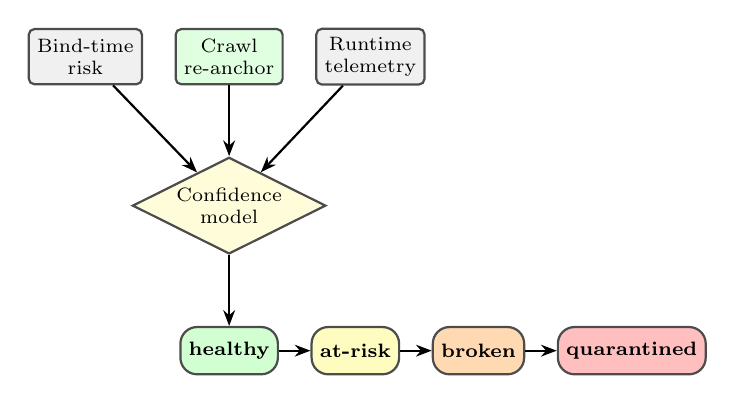
\begin{tikzpicture}[node distance=4mm]
\node[box, fill=black!6] (bind) {Bind-time \\ risk};
\node[net, right=of bind] (crawl) {Crawl \\ re-anchor};
\node[box, fill=black!6, right=of crawl] (tel) {Runtime \\ telemetry};
\node[decision, below=9mm of crawl] (conf) {Confidence \\ model};
\draw[flow] (bind) -- (conf);
\draw[flow] (crawl) -- (conf);
\draw[flow] (tel) -- (conf);
% ladder
\node[term, fill=green!18, below=9mm of conf] (h) {healthy};
\node[term, fill=yellow!25, right=4mm of h] (a) {at-risk};
\node[term, fill=orange!30, right=4mm of a] (b) {broken};
\node[term, fill=red!25, right=4mm of b] (q) {quarantined};
\draw[flow] (conf) -- (h);
\draw[flow] (h) -- (a);
\draw[flow] (a) -- (b);
\draw[flow] (b) -- (q);
\node[left=2mm of h, font=\scriptsize\itshape, align=right] {} ;
\end{tikzpicture}
\caption{Three independent detection channels feed a confidence model that maps each binding onto a four-state health ladder. A duplicate observation fails safe directly to \emph{quarantined}.}
\label{fig:channels}
\end{figure}

\subsection{Confidence Model and Status Ladder}
Every binding is assigned a confidence metric within the range [0,100] and categorized into one of four states. This state allocation prioritizes system stability. Duplicate or ambiguous observations result in binding quarantine, preventing the application of modifications to unverified targets. Bindings exhibiting minimal confidence are classified as broken, whereas moderate confidence levels or observed runtime failures yield an at-risk classification; all other valid states remain healthy. Legacy bindings lacking descriptors are categorized as unknown and retain a healthy status, preventing false positive alerts in the absence of explicit structural drift data.

\subsection{Classification Algorithm}
Upon re-resolving a descriptor, the crawler classifies the specific modification event to facilitate targeted recovery procedures, as detailed in Algorithm 1 and Fig. 3. A uniquely resolved anchor exhibiting a tag mutation is designated as a replacement. If the text mutates while the original content remains uniquely resolvable elsewhere, the event is classified as a move. Mutations failing these criteria are categorized as content conflicts. When an anchor fails to resolve entirely, fingerprint analysis differentiates authentic moves, characterized by identical tags and text located elsewhere, from absolute removals. Candidate elements presenting similar attributes but divergent text are classified as ambiguous, thereby precluding erroneous re-binding and prioritizing manual verification.

\begin{algorithm}
\renewcommand{\algorithmicrequire}{\textbf{Input:}}
\renewcommand{\algorithmicensure}{\textbf{Output:}}
\begin{algorithmic}[1]
\REQUIRE descriptor $d$, freshly parsed document tree $T$
\ENSURE  category, confidence, status
\STATE $E \leftarrow$ elements($T$)
\IF{$d.\mathit{weblay} \neq \emptyset$}
  \STATE $H \leftarrow \{e \in E : e[\text{data-weblay}] = d.\mathit{weblay}\}$
  \IF{$|H| = 1$}
    \STATE $h \leftarrow$ the unique element of $H$
    \RETURN verify($E,h,d$)
  \ELSIF{$|H| = 0$}
    \RETURN classifyMissing($E,d$)
  \ELSE
    \RETURN \textsc{ambiguous} \COMMENT{duplicate anchor}
  \ENDIF
\ENDIF
\STATE $P \leftarrow \{e \in E : \text{path}(e) = d.\mathit{path}\}$
\IF{$|P| = 1$}
  \STATE $p \leftarrow$ the unique element of $P$
  \RETURN verify($E,p,d$)
\ELSIF{$|P| > 1$}
  \RETURN \textsc{ambiguous}
\ELSE
  \RETURN classifyMissing($E,d$)
\ENDIF
\end{algorithmic}
\caption{Descriptor re-resolution (server-side).}
\label{alg:resolve}
\end{algorithm}

\begin{figure}[t]
\centering
\resizebox{\columnwidth}{!}{%
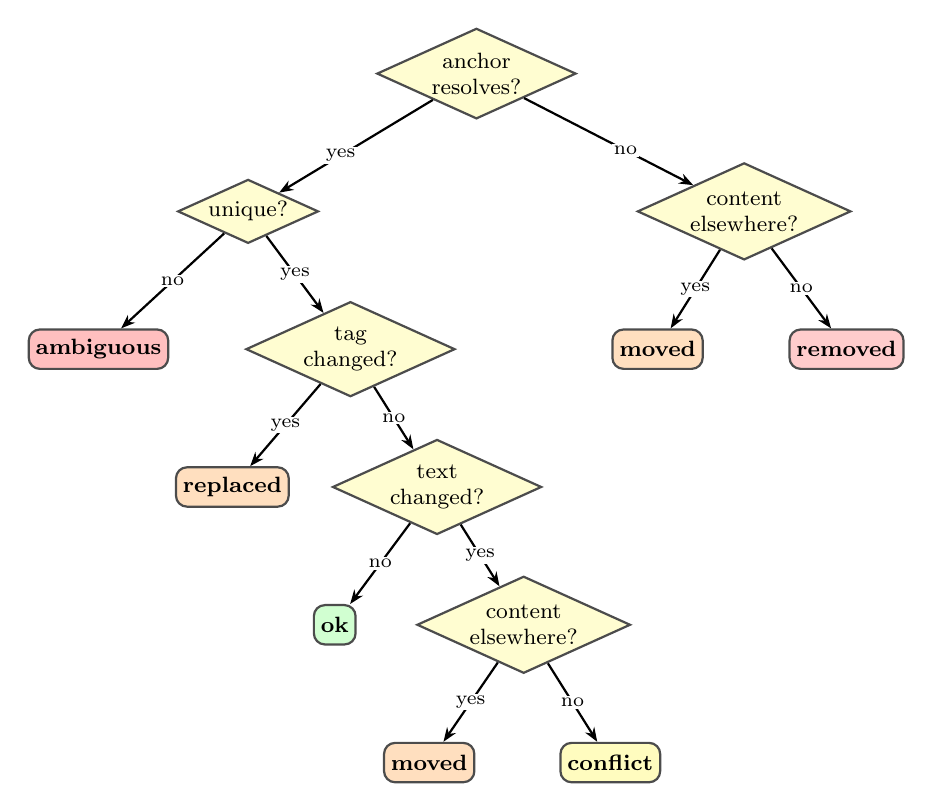
\begin{tikzpicture}[
  every node/.style={font=\footnotesize},
  dec/.style={diamond, aspect=2.2, draw=black!70, thick, fill=yellow!18,
              align=center, inner sep=1pt, minimum height=6mm},
  trm/.style={rectangle, rounded corners=4pt, draw=black!70, thick, align=center,
              font=\footnotesize\bfseries, inner sep=2.5pt, minimum height=5mm},
  e/.style={-{Stealth[length=1.8mm]}, thick},
  lbl/.style={font=\scriptsize, fill=white, inner sep=0.8pt},
]
% decisions
\node[dec] (res)  at (5.6, 0)     {anchor \\ resolves?};
\node[dec] (uniq) at (2.7,-1.75)  {unique?};
\node[dec] (fpN)  at (9.0,-1.75)  {content \\ elsewhere?};
\node[dec] (tag)  at (4.0,-3.5)   {tag \\ changed?};
\node[dec] (txt)  at (5.1,-5.25)  {text \\ changed?};
\node[dec] (fpR)  at (6.2,-7.0)   {content \\ elsewhere?};
% terminals
\node[trm, fill=red!25]    (amb)     at (0.8,-3.5)  {ambiguous};
\node[trm, fill=orange!25] (movedN)  at (7.9,-3.5)  {moved};
\node[trm, fill=red!20]    (removed) at (10.3,-3.5) {removed};
\node[trm, fill=orange!25] (repl)    at (2.5,-5.25) {replaced};
\node[trm, fill=green!18]  (ok)      at (3.8,-7.0)  {ok};
\node[trm, fill=orange!25] (movedR)  at (5.0,-8.75) {moved};
\node[trm, fill=yellow!25] (conf)    at (7.3,-8.75) {conflict};
% edges
\draw[e] (res)  -- node[lbl,pos=.6]{yes} (uniq);
\draw[e] (res)  -- node[lbl,pos=.6]{no}  (fpN);
\draw[e] (uniq) -- node[lbl]{no}  (amb);
\draw[e] (uniq) -- node[lbl]{yes} (tag);
\draw[e] (fpN)  -- node[lbl]{yes} (movedN);
\draw[e] (fpN)  -- node[lbl]{no}  (removed);
\draw[e] (tag)  -- node[lbl]{yes} (repl);
\draw[e] (tag)  -- node[lbl]{no}  (txt);
\draw[e] (txt)  -- node[lbl]{no}  (ok);
\draw[e] (txt)  -- node[lbl]{yes} (fpR);
\draw[e] (fpR)  -- node[lbl]{yes} (movedR);
\draw[e] (fpR)  -- node[lbl]{no}  (conf);
\end{tikzpicture}}
\caption{Classification decision path. A resolved-but-changed anchor is a move only if its original content still lives uniquely elsewhere; otherwise it is a content-conflict or, on tag change, a replacement.}
\label{fig:decision}
\end{figure}

\subsection{Redesign Detection}
If the failure rate of a page's verifiable bindings exceeds 40\% (with a minimum of three bindings), the page is classified as a redesign. Consequently, its edits are isolated and accompanied by a single "redesign-suspected" signal to prevent multiple unrelated alerts. Only bindings containing a descriptor are factored into this ratio, ensuring that legacy or telemetry-only bindings do not generate false redesign classifications.

\subsection{Recovery}\label{sec:recovery}
Each classified outcome corresponds to a specific corrective action. Table~\ref{tab:cures} enumerates the six change categories together with their interpretation and the recommended action for each. The system requires explicit operator authorization and does not automatically modify live pages. Consequently, an erroneous classification cannot silently corrupt a deployed page, and every applied action remains reversible through the page's version history.

\begin{table}[t]
\caption{Change category, its meaning, and the recommended cure.}
\label{tab:cures}
\centering
\footnotesize
\begin{tabular}{@{}p{1.5cm}p{3.0cm}p{2.3cm}@{}}
\toprule
\textbf{Category} & \textbf{Meaning} & \textbf{Recommended cure} \\
\midrule
Content-conflict & Source text under the edit changed & Reset (adopt source) \\
Moved & Element relocated in the tree & Re-bind to new position \\
Replaced & A different element now occupies the slot & Re-bind / reset \\
Removed & Target element is gone & Reset \\
Ambiguous & Several candidates or a look-alike & Harden / re-bind \\
Redesign & Mass drift across a page & Reset page or roll back \\
\bottomrule
\end{tabular}
\end{table}

The "Peek" function temporarily reverts all page overrides, including intra-session edits (for which original values are recorded upon initial interaction), allowing operators to view the unmodified state and subsequently restore edits without server communication. The "Reset" function eliminates an override and republishes, returning the element to its source markup while maintaining recoverability through version history. "Re-bind" directs the operator to designate the new location of the element, extracts a new descriptor, and transfers the edit. "Hardening" integrates a persistent data-weblay anchor, making the element resilient to renaming and reordering. Furthermore, the dashboard displays the health interface exclusively when issues are detected.

\section{Results and Discussion}\label{sec:eval}
\subsection{Experimental Setup}
Weblay was evaluated using a locally served, multi-section marketing site to test the complete pipeline. Edits were generated via the edit API using precise descriptors, and drift was simulated by mutating the underlying HTML. The production crawler was executed, and the subsequent health status was retrieved via the dashboard API. The server utilized a managed MongoDB backend. Six overrides were introduced to represent each drift category, supplemented by ten healthy overrides. This ensured that drift constituted a minority of the page content, thereby testing the per-category logic instead of the redesign heuristic.

\subsection{System Characteristics}
Table II details the static characteristics of the implementation. The primary bandwidth requirement for visitors is the 4.9 KB gzipped runtime; the 29 KB editor is not downloaded by standard end users.

\begin{table}[t]
\caption{Weblay implementation characteristics.}
\label{tab:sys}
\centering
\footnotesize
\begin{tabular}{@{}lr@{}}
\toprule
\textbf{Metric} & \textbf{Value} \\
\midrule
Visitor runtime (raw / gzip) & 12.3\,KB / 4.9\,KB \\
Editor bundle (raw / gzip, lazy) & 112\,KB / 29\,KB \\
Server core (Go, non-test) & 5{,}664 LOC \\
Connector (TypeScript) & 4{,}947 LOC \\
Storage backends & 3 (SQLite, Postgres, Mongo) \\
Change categories & 6 + unchanged \\
Health states & 4 \\
Detection channels & 3 \\
Automated tests & 26 \\
\bottomrule
\end{tabular}
\end{table}

\subsection{Detection Accuracy}
Table III presents the crawler's classification performance relative to the ground-truth mutations for each seeded binding. All fifteen bindings, consisting of five drifted and ten healthy controls, were accurately classified. The healthy controls maintained their status with maximum confidence, demonstrating a zero false-positive rate for the unmodified elements.

\begin{table}[t]
\caption{Detection results. Each drift category was introduced and classified through the production crawler.}
\label{tab:detect}
\centering
\footnotesize
\begin{tabular}{@{}llll@{}}
\toprule
\textbf{Introduced} & \textbf{Detected} & \textbf{Status} & \textbf{Conf.} \\
\midrule
Content-conflict & content-conflict & at-risk & 80\% \\
Removed & removed & broken & 15\% \\
Replaced (tag) & replaced & quarantined & 25\% \\
Moved (reorder) & moved & at-risk & 80\% \\
Ambiguous (dup) & ambiguous & quarantined & 30\% \\
$10\times$ unchanged & ok & healthy & 100\% \\
\midrule
\multicolumn{4}{@{}l@{}}{\textbf{Detection: 15 / 15 correct (0 false alarms)}} \\
\bottomrule
\end{tabular}
\end{table}

\subsection{Recovery Effectiveness}
Each drifted binding was then treated with its recommended corrective action, after which the page was re-crawled. Resetting cleared the two categories in which the edit no longer belongs, content-conflict and removed, by eliminating the override entirely. Re-binding resolved the relocatable cases, restoring the replaced and moved bindings to a healthy status at 100\% and 95\% confidence, respectively, while hardening returned the ambiguous binding to a healthy status at 100\% confidence. All five warnings were thereby cleared, reducing the site's aggregate open-issue count to zero.

\subsection{Practical Usage Across Site Archetypes}
To assess applicability beyond a single site, the detection pipeline was evaluated on three representative markup archetypes served locally: a \emph{semantic} static site authored with \texttt{data-weblay} anchors and stable identifiers; a \emph{framework} page emulating component-based output with generated identifiers, hashed class names, deep nesting, and no authored anchors; and a \emph{repeater} page comprising a grid of structurally identical product cards. For each archetype, one instance of each applicable drift category was introduced alongside unchanged controls, and the outcome was compared against ground truth. Table~\ref{tab:archetype} reports the results.

\begin{table}[t]
\caption{Detection across site archetypes. Accuracy is category precision; false positives are drift categories reported on unchanged controls.}
\label{tab:archetype}
\centering
\footnotesize
\begin{tabular}{@{}lcccc@{}}
\toprule
\textbf{Archetype} & \textbf{Anchors} & \textbf{Seeded} & \textbf{Accuracy} & \textbf{False pos.} \\
\midrule
Semantic  & authored & 7 & 100\% & 0 \\
Repeater  & authored & 8 & 100\% & 0 \\
Framework & none     & 2 & 50\%  & 0 \\
\bottomrule
\end{tabular}
\end{table}

The semantic and repeater archetypes were classified with full category precision and no false positives; in particular, the repeater's structurally identical cards did not induce spurious ambiguity because each card carried a distinct authored anchor. On the anchorless framework page, one of two cases degraded: a tag change was classified as \emph{removed} rather than \emph{replaced}. This is an expected consequence of relying on a structural path whose final step embeds the element tag: once the tag changes, the path no longer resolves and no same-tagged element with the original content remains, so the fingerprint search reports a removal. Notably, both outcomes place the binding in a \emph{broken} state that requires operator action, so the binding is still flagged with certainty; only the fine-grained category differs. This result quantifies the benefit of authored \texttt{data-weblay} anchors, which survive tag changes and thereby preserve category precision.

\subsection{Resilience to Structural Perturbation}
The central claim of the multi-signal descriptor is that redundant identity signals allow an edit to survive changes that would break any single signal. To test this directly, one edit on the semantic page was subjected to escalating perturbations, each designed to disable a specific signal, and the crawler's resolving signal was recorded from its reason codes. Table~\ref{tab:resilience} reports, for each perturbation, whether the edit remained correctly located and which signal resolved it.

\begin{table}[t]
\caption{Per-signal resilience. The edit remains correctly located even when both the structural path and the authored anchor are destroyed, because the content fingerprint resolves it.}
\label{tab:resilience}
\centering
\footnotesize
\begin{tabular}{@{}p{4.3cm}cp{2.1cm}@{}}
\toprule
\textbf{Perturbation} & \textbf{Located} & \textbf{Resolving signal} \\
\midrule
None (control)                         & yes & anchor \\
Structural path broken (element wrapped in a new \texttt{<div>}) & yes & authored anchor \\
Path broken \emph{and} anchor removed  & yes & content fingerprint \\
Sibling reordered before the target    & yes & anchor \\
\bottomrule
\end{tabular}
\end{table}

The edit remained correctly located under every perturbation. When the structural path was broken by inserting an intermediate element, the authored anchor still resolved the edit with full confidence. Critically, when both the structural path \emph{and} the authored anchor were removed, the content fingerprint alone re-located the element: the crawler reported \texttt{resolved-by-fingerprint} and classified the outcome as a move rather than a loss. This demonstrates the intended signal redundancy: no single point of failure exists between an edit and its element.

\subsection{Robustness to Build Churn}
A common source of spurious drift in selector-based tools is ordinary build churn, in which a framework regenerates hashed class names and component identifiers on every deployment without changing visible content. To measure Weblay's robustness, four edits were seeded on a page whose class names and identifiers were regenerated on each of five simulated rebuilds while the semantic content was held fixed. Across the resulting twenty binding checks, \textbf{zero} false alarms were recorded (false-alarm rate 0.0\%), because the descriptor excludes hashed-looking class tokens and framework-generated identifiers from its trusted signals.

\subsection{Client-Rendered Pages}
The rendering escalation was evaluated on a single-page-application shell whose initial HTML contains only an empty root element and a script that injects the edited content after load. A descriptor for an injected element does not resolve against the static response, since the element is absent; the same descriptor resolves to a healthy binding after the headless-rendering pass. The crawler therefore recovers content that a static fetch alone would report as removed, at the cost of one browser render for pages detected as client-rendered.

\subsection{Discussion}
The evaluation validated both the detection mechanism and the efficacy of the classifier's distinctions. Two seemingly plausible outcomes represent critical misclassifications that the multi-signal approach corrects: a reordered element occupying a reused slot, which naive text comparison misinterprets as an in-place content edit, and a removed element with a reused class, which is incorrectly identified as a relocation. Weblay classifies the former as moved (prompting a re-bind rather than a reset) and the latter as ambiguous (preventing erroneous re-anchoring to a look-alike element).

Two cost components must be distinguished. The re-resolution \emph{compute}, namely the tree walk that matches a descriptor against parsed HTML, was measured at approximately 4.7\,$\mu$s per descriptor on a forty-section page and is therefore negligible. The end-to-end \emph{persisted scan} latency is instead dominated by writing each binding's health record to the managed (remote) database, each write incurring a network round-trip. With one write per binding, this latency grew approximately linearly, from 1.6\,s at five bindings to 7.0\,s at forty ($\sim$135\,ms per binding). We therefore batch all of a page's health writes into a single bulk update; as Fig.~\ref{tab:latency} shows, this flattens the latency to roughly constant ($\sim$1.0 to 1.5\,s across 5 to 40 bindings), so scan cost now scales with the number of pages rather than the number of edits.

\begin{figure}[t]
\centering
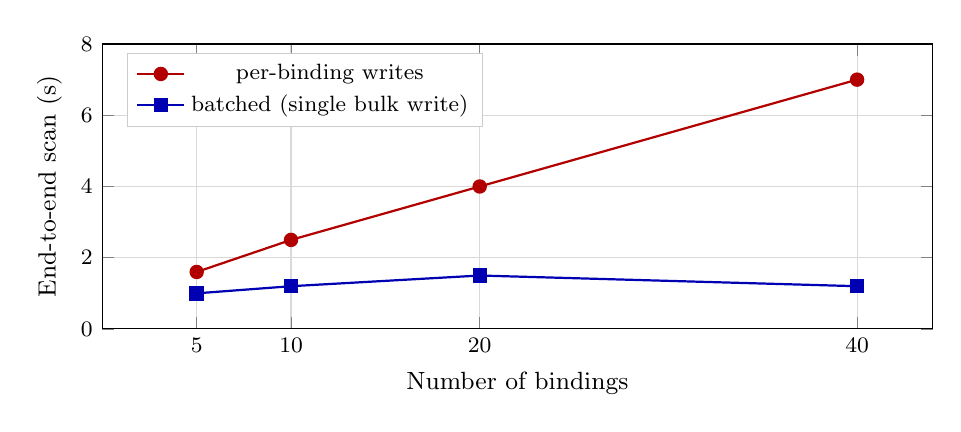
\begin{tikzpicture}
\begin{axis}[
  width=\columnwidth, height=5.2cm,
  xlabel={Number of bindings},
  ylabel={End-to-end scan (s)},
  xmin=0, xmax=44, ymin=0, ymax=8,
  xtick={5,10,20,40}, ytick={0,2,4,6,8},
  grid=both, grid style={gray!25}, major grid style={gray!30},
  tick label style={font=\footnotesize}, label style={font=\small},
  every axis plot/.append style={thick},
  legend style={font=\footnotesize, at={(0.03,0.97)}, anchor=north west, draw=gray!40},
]
\addplot[mark=*, mark size=2.2pt, color=red!70!black]
  coordinates {(5,1.6) (10,2.5) (20,4.0) (40,7.0)};
\addlegendentry{per-binding writes}
\addplot[mark=square*, mark size=2.2pt, color=blue!70!black]
  coordinates {(5,1.0) (10,1.2) (20,1.5) (40,1.2)};
\addlegendentry{batched (single bulk write)}
\end{axis}
\end{tikzpicture}
\caption{Crawl latency versus binding count (median of five runs, managed remote database). With one write per binding, latency grew approximately linearly at $\sim$135\,ms per binding; batching all of a page's writes into a single bulk update flattens it to roughly constant ($\sim$1.0 to 1.5\,s), removing the dependence on binding count.}
\label{tab:latency}
\end{figure}

\subsection{Threats to Validity}
The evaluation spans three markup archetypes and controlled perturbations rather than a longitudinal study of real-world redesigns, which may combine change categories in ways not captured here. Category precision was lower on anchorless, framework-generated markup, as noted above; generalizing this behavior requires a wider corpus of production frameworks. The crawling mechanism also requires the target site to be publicly accessible from a registered origin. Finally, runtime telemetry serves as a corroborating source but remains best-effort and vulnerable to ad-blocking interference.

\section{Conclusion and Future Work}\label{sec:conc}
This paper presented a method for persisting end-user visual edits as page markup evolves, storing each edit against a multi-signal descriptor and re-resolving it server-side into one of six change categories across three corroborating detection channels, each paired with a corrective action. In an end-to-end evaluation, all six categories were classified correctly across fifteen edits with no false positives on the unchanged set, and every flagged edit was cleared by its recommended action. These results indicate that combining multiple weak identity signals with server-side re-resolution can determine, offline and at scale, whether a stored edit remains applicable to a modified page and, if not, why.

Several directions remain for future work. First, automatic hardening could proactively propose durable anchors during the editing phase rather than solely as a corrective measure. Second, a deploy-webhook trigger, already implemented, initiates re-resolution upon site modification rather than at fixed intervals, reducing detection latency from the crawl interval to under one second in informal measurements; integrating it directly with common continuous-integration pipelines is a natural extension. Finally, augmenting the descriptor with lightweight visual features could further disambiguate elements that share identical tags and attributes but differ visually.

\begin{thebibliography}{00}
\bibitem{webflow} Webflow, Inc., ``Webflow: visual web development platform.'' [Online]. Available: https://webflow.com/ (accessed Aug. 2026).
\bibitem{wp} WordPress, ``Block Editor Handbook.'' [Online]. Available: https://developer.wordpress.org/block-editor/ (accessed Aug. 2026).
\bibitem{optimizely} Optimizely, ``Web experimentation.'' [Online]. Available: https://www.optimizely.com/products/web-experimentation/ (accessed Aug. 2026).
\bibitem{selfheal} M. Leotta, A. Stocco, F. Ricca, and P. Tonella, ``Using multi-locators to increase the robustness of web test cases,'' in \emph{Proc. IEEE 8th Int. Conf. Softw. Testing, Verification and Validation (ICST)}, 2015, pp. 1-10, doi: 10.1109/ICST.2015.7102611.
\bibitem{robula} M. Leotta, A. Stocco, F. Ricca, and P. Tonella, ``ROBULA+: an algorithm for generating robust XPath locators for web testing,'' \emph{J. Softw. Evol. Process}, vol. 28, no. 3, pp. 177-204, 2016, doi: 10.1002/smr.1771.
\bibitem{healenium} EPAM, ``Healenium: self-healing library for Selenium-based tests.'' [Online]. Available: https://healenium.io/ (accessed Aug. 2026).
\bibitem{xydiff} G. Cob\'ena, S. Abiteboul, and A. Marian, ``Detecting changes in XML documents,'' in \emph{Proc. 18th Int. Conf. Data Engineering (ICDE)}, 2002, pp. 41-52, doi: 10.1109/ICDE.2002.994696.
\bibitem{vdom} Meta, ``Reconciliation,'' React documentation. [Online]. Available: https://legacy.reactjs.org/docs/reconciliation.html (accessed Aug. 2026).
\bibitem{shadowdom} WHATWG, ``DOM Standard,'' \S 4.8 (Shadow trees). [Online]. Available: https://dom.spec.whatwg.org/\#shadow-trees (accessed Aug. 2026).
\bibitem{djb2} D. J. Bernstein, ``djb2,'' hash function posted to the comp.lang.c newsgroup, 1991.
\bibitem{swr} M. Nottingham, ``HTTP Cache-Control Extensions for Stale Content,'' RFC 5861, IETF, May 2010, doi: 10.17487/RFC5861.
\bibitem{ssrf} OWASP, ``Server Side Request Forgery Prevention Cheat Sheet.'' [Online]. Available: https://cheatsheetseries.owasp.org/cheatsheets/Server\_Side\_Request\_Forgery\_Prevention\_Cheat\_Sheet.html (accessed Aug. 2026).
\end{thebibliography}

\end{document}
